\documentclass[11pt]{report}

\setlength{\parindent}{0em}
\setlength{\parskip}{0.5em}

\usepackage{url}
\usepackage{amsmath}
\usepackage{cleveref}
\usepackage{ntheorem}
\usepackage[a4paper]{geometry}

\begin{document}

\title{Credal Classification of Automobile Risk}
\author{Ben Willis}
\maketitle

\begin{abstract}
	This project investigates how a credal classifier can be applied to the problem of determining automobile insurance risk. Currently automobiles are assigned a risk rating by an expert who takes in to account various attributes of a vehicle. We build a classifier capable of emulating the experts assessments.
\end{abstract}

\tableofcontents

\chapter{Introduction}

Classifiers have many applications in the finance industry ranging from financial trading \cite{Gerlein16} to credit card fraud detection \cite{Pozzolo15}.
We will study the problem of determining the risk to an insurer of a vehicle.
Initially we will learn from an experts classification of risk.
We will then examine how both the expert's and our classifications compare to the actual normalised loss to the insurer of each vehicle.

Classification is the problem of identifying which class an object belongs to.
Each object can be distinguished by a set of properties know as features and each object belongs to a single class.
A classifier is an algorithm which, given previous observations and their classes, can determine which class a new observation belongs to \cite{Theodoridis03}.
There are many applications of classifiers including image recognition, sentiment analysis and medical diagnosis.

A credal classifier is a special type of classifier.
Instead of returning a single class for a new observation it returns a set of classes.

The data set we will be analysing contains vehicular information from 205 automobiles.
Its features include dimensions, engine specifications and vehicle characteristics.
It also contains an expert's assessed risk to the insurer of the vehicle on an integer scale of -2 to 3 with 3 being most risky and -2 being least risky.
In addition to the technical information and the experts assessment, the data set also contains the normalized loss to the insurer.
This ranges from 65 to 256 and is normalized for all vehicles within a particular size classification (two-door small, station wagons, etc.) and represents the average loss per car per year \cite{Automobile}.
\chapter{Naive Bayes Classifier}

To begin with we will define a simple probabilistic classifier known as the naive Bayes classifier.
This classifier is based on Bayes theorem:
\begin{equation} \label{Bayes Theorem}
	P(A \mid B) = \frac{P(B \mid A)P(A)}{P(B)}
\end{equation}
This result was first described in Thomas Bayes' posthumous work ``An Essay towards solving a Problem in the Doctrine of Chances'' \cite{Bayes63}.
A Bayesian approach to artificial intelligence has been used since the 1960s, especially in a medical setting \cite{Russell03}.
The naive Bayes classifier which we will study in this chapter has it's roots in information retrieval \cite{Lewis98} however has been applied to  many other problems including breast cancer diagnosis \cite{Dumitru09} and text analysis \cite{Nigam98}.


\section{Basic Classifier}

To help explain how the naive Bayes classifier works we will introduce a new data set from a remote sensing study.
The study measured spectral information in the green, red and infrared wavelengths on three separate dates of $523$ different areas of forest in Japan.
In total each observation has nine continuous attributes and falls in to one of four possible classes: Sugi forest, Hinoki forest, Mixed deciduous forest and other non-forest land.
This data set was chosen as it contained a large number of observations and demonstrates a situation where this type of classifier works well.

Formally, let us denote the class variable by $C$, taking values from the set $\mathcal{C} = \{0,1,2,3\}$ for each of the four types of forest.
We measure 9 features $A_1,\dots,A_9$ which we discretize so that they all take values from the set $\mathcal{A} = \{0,\dots,9\}$.
The observations of the variables are denoted by $c$ and $a_1,\dots,a_9$ respectively.

We are interested in the probability of a forest being of type $c$ given sensor readings $\mathbf{a}$ i.e. $P(c \mid \mathbf{a})$.
Using Bayes theorem we can rewrite this as:
\begin{equation} \label{bayes}
	P(c \mid \mathbf{a}) = \frac{P(c)P(\mathbf{a} \mid c)}{P(\mathbf{a})}
\end{equation}

Moreover we can make use of the naivety assumption.
The naivety assumptions states that the attributes are conditionally independent given the class.
In the context of this data set we are assuming the sensor readings are conditionally independent given the type of forest.
This assumption may not necessarily be accurate however it simplifies the problem.
We can therefore write the probability of observing an object with attributes $a_1, \dots\ a_9$ given it is in class $c$ as:
\begin{equation} \label{naivety}
	P(\mathbf{a} \mid c) = \prod_{i=1}^9 P(a_i \mid c)
\end{equation}

Note that $P(\mathbf{a})$ is independent of $c$ and is just a scaling constant.
So by bringing together \cref{bayes,naivety} we can write:
\begin{equation}
	P(c \mid \mathbf{a}) \propto P(c)\prod_{i=1}^{9}P(a_i \mid c)
\end{equation}

To turn this into a classifier we need a way to decide which class a forest falls into based on these probabilities.
We can introduce a \textit{loss function} to allow us to choose the class.
A standard choice is the 0-1 loss function defined as:
\begin{equation}\label{0-1_loss_function}
	L(c, \hat{c}) = 
	\begin{cases}
		0 & \text{if}\ c = \hat{c} \\
		1 & \text{otherwise}
	\end{cases}
\end{equation}
This function assigns a loss of 1 to any wrong classification regardless of the class that is assigned. 
Under this loss function we can write the expected loss as:
\begin{equation}
	E(L) = \sum L(c, \hat{c})P(c \mid \mathbf{a}) = 1 - P(\hat{c} \mid \mathbf{a})
\end{equation}
So to minimize our expected loss we choose:
\begin{equation} \label{map_estimate}
	\hat c = \arg\max_{c \in \mathcal{C}} P(c)\prod_{i=1}^{k}P(a_i \mid c)
\end{equation}
This is known as the maximum a posteriori (MAP) estimate.
We will investigate other options for the loss function later on in this report.

Now that we have our method for making our decision we need to estimate the required probabilities.

To do so we parametrise these probabilities.
We denote the unknown chances of observing an object in class $c$ by $\theta_c$ and the chance of observing an object in class $c$ with attributes $\mathbf{a}$ by $\theta_{\mathbf{a}, c}$.
Similarly we denote the conditional chances of observing an individual attribute $a_i$ and a set of attributes $\mathbf{a}$ given $C=c$ by $\theta_{a_i \mid c}$ and $\theta_{\mathbf{a} \mid c}$ respectively.

Now we have parametrised the probabilities, we wish to estimate we can consider the likelihood function for $\mathbf{\theta}$, the vector whose elements are the chances $\theta_{c}$ and $\theta_{a_i \mid c}$.
Using our data we denote the frequencies of objects in each class $c$ by $n(c)$ and the number of objects in class $c$ with attribute $a_i$ by $n(a_i, c)$.
For example, returning to the forest type data set, the number of observations of class $0$ is $158$ so $n(0) = 158$.
Note that $\sum_{c \in \mathcal{C}}n(c) = N$ and $\sum_{a_i \in \mathcal{A}_i}n(a_i, c) = n(c)$.
We then consider the vector $\mathbf{n}$ which contains these frequencies.

We can derive the likelihood function for these theta chances given the frequencies described above:
\begin{align} \label{likelihood}
	l(\mathbf{\theta} \mid \mathbf{n}) & =  \prod_{c \in \mathcal{C}} \prod_{\mathbf{a} \in \mathbf{\mathcal{A}}} \theta_{\mathbf{a}, c}^{n(\mathbf{a}, c)} \\
	& = \prod_{c \in \mathcal{C}} \prod_{\mathbf{a} \in \mathbf{\mathcal{A}}} \left[ \theta_{c}^{n(\mathbf{a}, c)} \theta_{\mathbf{a} \mid c}^{n(\mathbf{a}, c)} \right] \\
	& = \prod_{c \in \mathcal{C}} \left[ \theta_{c}^{\sum_{\mathbf{a} \in \mathbf{\mathcal{A}}} n(\mathbf{a}, c)} \prod_{\mathbf{a} \in \mathbf{\mathcal{A}}} \prod_{i=1}^k \theta_{a_i \mid c}^{n(\mathbf{a}, c)} \right] \\
	& \propto \prod_{c \in \mathcal{C}} \left[ \theta_c^{n(c)} \prod_{i=1}^k \prod_{a_i \in \mathcal{A}_i} \theta_{a_i \mid c}^{n(a_i, c)} \right]
\end{align}

Now we want to estimate these probabilities.
A simple estimate for these parameters is the maximum likelihood estimate (MLE).
To find the MLE first we take the log likelihood:
\begin{equation}
	L(\mathbf{\theta} \mid \mathbf{n}) \propto \sum_{c \in \mathcal{C}}  n(c)log(\theta_c) + \sum_{c \in \mathcal{C}} \sum_{i=1}^k \sum_{a_i \in \mathcal{A}_i} n(a_i, c) log(\theta_{a_i \mid c}) 
\end{equation}
We want to maximise the likelihood function.
To do so we maximise each part of the log likelihood function which we will do so through the use of Lagrange multipliers.
This is a strategy for finding local maxima and minima of a function subject to constraints.

For the $\theta_c$ parameters we want to maximise:
\begin{equation}
	f(\mathbf{\theta}, \mathbf{n}) = \sum_{c \in \mathcal{C}}  n(c)log(\theta_c)
\end{equation}
under the constraint:
\begin{equation}\label{theta_c constraint}
	g(\mathbf{\theta}, \mathbf{n}) = \sum_{c \in \mathcal{C}}  \theta_c - 1 = 0
\end{equation}
This gives us our Lagrangian:
\begin{equation}
	\mathcal{L}(\mathbf{\theta}, \mathbf{n}, \lambda) = \sum_{c \in \mathcal{C}}  n(c)log(\theta_c) - \lambda(\sum_{c \in \mathcal{C}}  \theta_c - 1)
\end{equation}

Differentiating with respect to $\theta_c$ we have:
\begin{equation}
	\nabla_{\theta_c} \mathcal{L}(\mathbf{\theta}, \mathbf{n}, \lambda) = \frac{n(c)}{\theta_c} - \lambda
\end{equation}

Setting this to zero and using the constraint in \cref{theta_c constraint} we have maximum likelihood estimate:
\begin{equation}
	\hat\theta_c = \frac{n(c)}{N}
\end{equation}
This is just the relative frequency of observations that fall into that class.
Returning to our example data set we have $N=523$ and $n(0)=158$ so $\hat\theta_0 = \frac{158}{523} \approx 0.302$

Similarly for the $\theta_{a_i \mid c}$ parameters we want to maximize:
\begin{equation}
	f(\mathbf{\theta}, \mathbf{n}) = \sum_{c_i \in \mathcal{A}_i} n(a_i, c) log(\theta_{a_i \mid c})
\end{equation}
for each $c \in \mathcal{C}$ and $i \in \{1,\dots,k\}$ under the constraint:
\begin{equation}
	g(\mathbf{\theta}, \mathbf{n}) = \sum_{a_i \in \mathcal{A}_i}  \theta_{a_i \mid c} - 1 = 0
\end{equation}
We again solve this using the Lagrangian to find the maximum likelihood estimate:
\begin{equation}
	\hat\theta_{a_i \mid c} = \frac{n(a_i, c)}{n(c)}
\end{equation}

We can now estimate the required probabilities and hence have our naive Bayes classifier.
First we estimate the probabilities by taking the maximum likelihood estimate for their parametrisation:
\begin{align}
	P(c) & = \frac{n(c)}{N} \\
	P(a_i \mid c) & = \frac{n(a_i, c)}{n(c)}
\end{align}
Then for an object with an unknown class we choose the MAP estimate given in \cref{map_estimate}.

\section{Diagnostics}

To measure how successful our classifier is we will initially use a technique known as \textit{k-fold cross validation}.
In $k$-fold cross validation we split our dataset into $k$ equally sized groups.
Then for each of these group we train the classifier on all the other groups then test it on the excluded group.
We then average all these measurements to return an estimate for the measurement of our classifier.

The choice of $k$ leads to different types of cross validation.
A special case of cross validation is when $k=n$ (the number of observations).
This is knowns as leave-one-out cross validation \cite{Priddy05}.

Initially we will consider two metrics.
The first is accuracy, this is the percentage of correctly classified objects restricted to the case where there is a single MAP estimate.
The seconds is indeterminate classifications, this is percentage of objects with no unique MAP estimate for their class and usually occurs when $P(c \mid \mathbf{a}) = 0$ for all $c \in \mathcal{C}$.

The accuracy of the classifier is 81.77\% and the percentage of unclassified objects is 2.04\% on the forest data set, using 10-fold cross validation.

Previous work carried out by Johnson et al. \cite{Johnson12} on the data set aimed to improve their classification by weighting training data based on geographical distance.
They used SVMs (Support Vector Machines) to classify the forests and recorded an accuracy of 85.9\%.
This indicates that our relatively simple NBC can still achieve a high degree of accuracy.

\section{Application to Automobile Data set}

Now we've seen an application of the NBC to a straightforward data set we want to apply it to our insurance problem.

To make our automobile data appropriate for this method we discretize the continuous variables into $10$ bins with an equal frequency.

Unlike in the trees data set, in this data set we have objects with missing values for attributes.
We have no mechanism for considering these so we must discard these observations for now.
This reduces our data set from 205 observations to 193 observations.

As before we carry out 10-fold cross validation for the two metrics.
The accuracy of our classifier is 59.95\% on the automobile data set.
This is considerably worse than the example forest data set, moreover 22.45\% of the objects were not classified.

Clearly the classifier performs better on the forest type dataset than on the automobile data set.
There are also general failings in our classifier we can fix to improve its accuracy for both data sets.

Firstly our classifier falls down if there are no observations with attribute $a_j$ and class $c$ in our training set.
In these case the maximum likelihood estimate for $\theta_{a_j \mid c}$ is $0$.
This estimate leads to $P(c \mid \mathbf{a}) = 0$ and would rule out assigning any objects with the attribute $a_j$ to class $c$.
This is especially problematic for small sets of data and contributes to the large percentage of indeterminate classifications we saw when applying the classifier to the automobile insurance data set.
We can tackle this by introducing a prior distribution for the theta chances.

One thing that the automobile data set has that the forest type data set doesn't is missing values.
By discarding the objects with missing values we throw away $20$ observations from an already small data set.
If we could make use of these incomplete observation we should be able to improve our classifier.

We can also make use of the structure in the automobile data set's ordered classes.
The accuracy metric does not take into account how close the classification is.
For example if the true class is 2 an assigned class of 1 should be considered better than an assigned class of -2.
The 0-1 loss function also does not take this into account and a better choice of loss function may prove beneficial.


\chapter{Corrected NBC with Dirichlet Prior}

\section{Theory}

We return to our likelihood function \cref{likelihood} for our theta variables.
We can introduce a prior distribution for these parameters and then consider the posterior distribution.

The Dirichlet distribution is the multinomial extension of the beta distribution for $\theta_1,\dots,\theta_k$ where $\theta_i \in (0,1)$ and $\sum_{i=1}^k \theta_i = 1$ with probability density function:
\begin{equation} \label{dirichlet_pdf}
	f(\theta_1,\dots,\theta_k \mid s, t(1),\dots,t(k)) \propto \prod_{i=1}^k \theta_i^{st(i) - 1}
\end{equation}
where $s > 0$ and each $t(i)>0$ such that $\sum_{i=1}^{k}t(i) = 1$.

We introduce a distribution that is similar to our likelihood as our prior density:
\begin{equation} \label{prior}
	f(\mathbf{\theta} \mid \mathbf{t}, s) \propto \prod_{c \in \mathcal{C}} \left[ \theta_c^{st(c) - 1} \prod_{i=1}^k \prod_{a_i \in \mathcal{A}_i} \theta_{a_i \mid c}^{st(c, a_i) - 1} \right]
\end{equation}
This is in the same form as the likelihood however each $n(\cdot)$ is replaces by $st(\cdot) - 1$.
$s > 0$ is a fixed constant and we have the following constraints on $t(\cdot):$
\begin{align}\label{prior_constraints}
	\sum_{c \in \mathcal{C}} t(c) & = 1 \\
	\sum_{a_i \in \mathcal{A}_i} t(a_i, c) & = t(c) && \forall i, c \\
	t(a_i, c) & > 0 && \forall i, a_i, c
\end{align}

This distribution is the conjugate prior for the likelihood function \cref{likelihood}.
When we multiply our likelihood by this prior density we get a posterior in the same family as this prior.
If the prior has hyper parameters $st(\cdot)$ the posterior will have hyper parameters $st(\dot) + n(\cdot)$.

We can now estimate the parameters by taking the posterior expectation e.g.
\begin{equation}
	E(\theta_c|\mathbf{n},s,\mathbf{t})=\hat{\theta_c} = \frac{n(c) + st(c)}{N + s}
\end{equation}

We estimate:
\begin{align}
	P(c) & \text{ by } \frac{n(c) + st(c)}{N + s} \\
	P(a_i \mid c) & \text{ by } \frac{n(a_i, c) + st(a_i, c)}{n(c) + st(c)}
\end{align}

\section{Application}

To apply this classifier to our data set we need to choose the hyper parameters of the prior distribution.
We note that $s$ affects the speed at which our classifier learns and $t(\cdot)$ represents our beliefs for $\theta_\cdot$.
To comply with the constraints \ref{prior_constraints} let us set:
\begin{align}
	s & = 1 \\
	t(c) & = \frac{1}{|C|} \\
	t(a_i, c) & = \frac{1}{|A_i||C|}
\end{align}

Previously we've considered the accuracy of our classifier.
An alternative metric is the mean squared error of our estimate.
\begin{equation}
	\text{MSE} = \frac{1}{n}\sum_{i=1}^n(\hat{c_i} - c_i)^2
\end{equation}

\begin{center}
	\begin{tabular}{ c|c c c c c c }
		              & Accuracy & MSE   & Failed Classifications\\
		\hline
		NBC           & 59.95\%  & 2.823 & 22.45\% \\
		Corrected NBC & 68.17\%  & 0.689 & 0\%
	\end{tabular}
\end{center}

This again shows an improvement over the previous classifier.

\section{Conclusions}
\chapter{Alternate Loss Functions}

In chapter two we introduced the idea of a loss function.
We used the 0-1 loss function to make decision of which class to place an object in given its attributes.
In this chapter we will investigate some alternate loss functions that make better use of the structure of the insurance problem.

When classifying the insurance risk of a vehicle we return a class on an integer of scale of -2 to 3.
The 0-1 loss function assigns a loss of 1 to any risk rating that is not the true risk rating, regardless of how close it is.
We will test alternate choices for the loss function by measuring the accuracy and mean squared error.
We will use the expected posterior estimates with the uniform prior as described in the previous chapter.

\section{The Loss Functions}
\subsection{0-1 Loss Function}
Previously we considered the 0-1 loss function.
To recap this is defined by:
\begin{equation}
	L(c, \hat{c}) = 
	\begin{cases}
		0 & \text{if}\ c = \hat{c} \\
		1 & \text{otherwise}
	\end{cases}
\end{equation}

The expected loss is:
\begin{equation}
	E(L) = \sum_{c \in \mathcal{C}} L(c, \hat{c})P(c \mid \mathbf{a}) = 1 - P(\hat{c} \mid \mathbf{a})
\end{equation}

So to minimize our expected loss we choose:
\begin{equation}
	\hat c = \arg\max_{c \in \mathcal{C}} P(c)\prod_{i=1}^{k}P(a_i \mid c)
\end{equation}
This is known as the maximum a posteriori (MAP) estimate.

\subsection{Squared Differences}
The squared differences loss function is defined as:
\begin{equation}
	L(c, \hat{c}) = (c - \hat{c})^2
\end{equation}
This assigns greater loss to risk ratings that are further away from the true value.

For this function the expected loss is:
\begin{equation}
	E(L) = \sum_{c \in \mathcal{C}} (c - \hat{c})^2P(c \mid \mathbf{a}) 
\end{equation}

Differentiating this with respect to $\hat{c}$ gives:
\begin{equation}
	\frac{\partial}{\partial \hat{c}} E(L) = \sum_{c \in \mathcal{C}} (-2c + 2\hat{c})P(c \mid \mathbf{a}) 
\end{equation}
Setting this equal to zero gives:
\begin{align}
	\sum_{c \in \mathcal{C}} cP(c \mid \mathbf{a}) & = \sum_{c \in \mathcal{C}} \hat{c}P(c \mid \mathbf{a}) \\
	E(c \mid \mathbf{a}) & = \hat{c}
\end{align}
So the estimate which minimizes the loss function is the expected class.
In the context of our problem the estimated class must be an integer, however this expected value may not be.

\subsection{Absolute Difference}
Finally we have the absolute difference loss function:
\begin{equation}
	L(c, \hat{c}) = | c - \hat{c} |
\end{equation}
Once again this assigns greater loss to risk ratings that are further away from the true value.

For this function the expected loss is:
\begin{align}
	E(L) & = \sum_{c \in \mathcal{C}} |c - \hat{c}|P(c \mid \mathbf{a}) \\
	     & = \sum_{c \leq \hat{c}} (\hat{c} - c)P(c \mid \mathbf{a}) - \sum_{c \geq \hat{c}} (\hat{c} - c)P(c \mid \mathbf{a})
\end{align}

Differentiating this with respect to $\hat{c}$ gives:
\begin{equation}
	\frac{\partial}{\partial \hat{c}} E(L) = \sum_{c \leq \hat{c}} P(c \mid \mathbf{a}) - \sum_{c \geq \hat{c}} P(c \mid \mathbf{a})
\end{equation}
Setting this equal to zero gives:
\begin{align}
	\sum_{c \leq \hat{c}} P(c \mid \mathbf{a}) & = \sum_{c \geq \hat{c}} P(c \mid \mathbf{a}) \\
	P(c \leq \hat{c} \mid \mathbf{a}) & = P(c \geq \hat{c} \mid \mathbf{a})
\end{align}
So the estimate that minimizes expected loss for this loss function is the median value.
This may be difficult to define on our data set.
For example suppose class -3 had $P(C = -2 \mid \mathbf{a}) = 0.5 = P(C=3 \mid \mathbf{a})$ then any class could reasonably be considered the median and therefore minimize our expected loss.
When more than one risk rating could be reasonably considered the median we will choose one at random.

\section{Application}
We will now apply these loss functions to our auto mobile data set and measure accuracy and mean squared error.
We will also investigate how often the assigned classes agree.

Once again we discretize and discard vehicles with missing attributes.

As the expected posterior estimates perform better than the maximum likelihood estimates we shall use these to estimate the required probabilities.
We will also use the uniform hyper parameters and set $s=1$.

Using 10-fold cross validation our various loss functions perform as follow.

\begin{center}
\begin{tabular}{l|c c}
	Loss Function       & Accuracy & MSE   \\
	\hline
	0-1                 & 68.59\%  & 0.642 \\
	Squared Difference  & 67.48\%  & 0.594 \\
	Absolute Difference & 68.34\%  & 0.635 \\
\end{tabular}
\end{center}

Note the similarity between the 0-1 loss function and the absolute difference loss function.
The squared difference loss function performs slightly worse in the accuracy metric however scores better for MSE.

We can also look at the percentage of time each loss function agrees:
\begin{center}
\begin{tabular}{l|c c c}
	Loss Function       & 0-1     & Squared Difference & Absolute Difference   \\
	\hline
	0-1                 & 100\% & 95.85\% & 99.48\% \\
	Squared Difference  & - & 100\% & 96.37\%\\
	Absolute Difference & - & - & 100\% \\
\end{tabular}
\end{center}

This confirms that the 0-1 loss function and absolute differences loss function assign classes in a very similar manner.
This is due to their often being a $\hat{c} \in \mathcal{C}$ such that $P(\hat{c} \mid \mathbf{a})$ that is much greater than for other choices of $c$ other.
When this is the case $\hat{c}$ is the choice for the 0-1 loss function.
Additionaly if it is greater than 0.5, which is often the case, it is the only choice for the median of the data set and hence is the absolute difference loss functions choice.

The squared difference loss function differs from these two slightly as it is more skewed by outliers.
Consider the case $P(C=-2\mid \mathbf{a})=0.6, P(C=3\mid \mathbf{a})=0.4$ then the expectation for $C$ is $0$ while both the 0-1 and absolute loss functions will choose -2.

\newcommand{\sn}[2]{\ensuremath{{#1}\times 10^{#2}}}

\chapter{Imprecise Prior}

When estimating the probabilities for our classifier we take in to account our prior beliefs for them and the likelihood given a set of observations.

When we initially chose our prior distribution we chose the parameters in \cref{initial prior} such that they follow the principal of indifference.
However as previously mentioned this prior does not truly represent our lack of prior knowledge about the parameters.
We need a way to represent this lack of knowledge and acknowledge that our estimates for the probabilities depend on this prior.

\section{Imprecise Dirichlet Model}

The imprecise Dirichlet model is a model for this lack of knowledge introduced by Walley \cite{Walley96}.
Instead of using a single prior distribution to represent our beliefs about the unknown parameters we use a set of prior distributions.

Suppose our objects had no attributes but we are still interested in classifying the object.
In the imprecise Dirichlet models the prior distributions are Dirichlet distributions with parameters $(s, \mathbf{t})$ such that $\sum_{c \in \mathcal{C}} t(c) = 1$.
The distributions for the likelihood are multinomial so:
\begin{equation}
	f(\mathbf{n} \mid \mathbf{\theta}) \propto \prod_{c \in \mathcal{C}} \theta_c^{n(c)}
	\qquad
	f(\mathbf{\theta} \mid s, \mathbf{t}) \propto \prod_{c \in \mathcal{C}} \theta_c^{st(c) - 1}
\end{equation}
Then the posterior distribution is of the form:
\begin{equation} \label{dirichlet_pdf}
	f(\mathbf{\theta} \mid \mathbf{n}, s, \mathbf{t}) \propto \prod_{c \in \mathcal{C}} \theta_c^{n(c) + st(c) - 1}
\end{equation}
which is also a Dirichlet distribution with parameters $(N+s, \frac{\mathbf{n}+s\mathbf{t}}{N+s})$.
We can then take the posterior expectation for the theta chances giving:
\begin{equation}
	P_t(c) = E(\theta_c \mid \mathbf{n}, s, \mathbf{t}) = \frac{n(c)+st(c)}{N+s}
\end{equation}
Note this is a function of $t(c)$ which allow us to obtain upper and lower estimates for for probabilities by varying $t(c)$:
\begin{align}
	\overline{P}(c) & = \frac{n(c)+s}{N+s} & (t(c) \rightarrow 1) \\
	\underline{P}(c) & = \frac{n(c)}{N+s}  & (t(c) \rightarrow 0)
\end{align}

Zaffalon applied this method of imprecise priors to the problem of classification.
We will use a set of the prior distributions of the form in \cref{prior} for a fixed value of $s$.
The parameter $s$ represents the strength of our prior beliefs and determines how quickly our classifier learns.

\section{Imprecise Probabilities}

Using this model we can find the upper and lower bounds for each posterior expectation based on different prior distributions.
Recall that we estimate the probabilities by taking the expectation of the posterior distribution and that these estimates depend on $\mathbf{t}$ i.e.:
\begin{align}
	P_t(c) & = E(\theta_c \mid \mathbf{n},s,\mathbf{t}) = \frac{n(c) + st(c)}{N + s} \\
	P_t(a_i \mid c) & = E(\theta_{a_i \mid c} \mid \mathbf{n},s,\mathbf{t}) = \frac{n(a_i, c) + st(a_i, c)}{n(c) + st(c)}
\end{align}
We can then use these to find upper and lower estimates for the probabilities over all values of $\mathbf{t}$ in our prior model.
For our distributions the upper and lower bounds are given by:
\begin{align}
	\overline{P}(c) & = \frac{n(c) + s}{N+s} \\
	\underline{P}(c) & = \frac{n(c)}{N+s}
\end{align}
These occur when we use the prior distributions with $t(c) \rightarrow 0$ and $t(c) \rightarrow 1$ respectively.

Similarly we have:
\begin{align}
	\overline{P}(a_i \mid c) & = \frac{n(a_i, c) + s}{n(c)+s} \\
	\underline{P}(a_i \mid c) & = \frac{n(a_i, c)}{n(c)+s}
\end{align}
These occur when we use the prior distributions with $t(c) \rightarrow 1$, $t(a_i, c)\rightarrow1$ and $t(c) \rightarrow 1$, $t(a_i, c)\rightarrow0$ respectively.

Let's start by comparing how our classifier behaves if we assume the true probability is at each end of the interval.
We will use the 0-1 loss function for the decision method and estimate each probability $P(\cdot)$ to be either the upper or lower probability of our interval.
We will measure accuracy and indeterminate classifications as before.

\begin{center}
	\begin{tabular}{l|c c}
	                & Accuracy & Indeterminate Assignments \\
	\hline
	Lower Estimates & 62.17\%  & 20.02\%            \\
	Upper Estimates & 40.09\%  & 0\%                \\
	\end{tabular}
\end{center}

Neither of these offer a sufficient classification.
There are often no observations of an attribute with a particular class which is why the lower estimates returns indeterminate classifications despite a reasonable accuracy for this data set.
On the other had the upper estimates have a terrible accuracy.

\section{Simple Credal Classifier}
Alternatively we can turn our classifier into a credal classifier.
A credal classifier assigns a set of classes as opposed to a single class to an object.

Recall the MAP estimate for the risk rating of a vehicle given by \cref{map}.
We say that a class $c'$ is dominated by $c''$ if:
\begin{equation}\label{Credal Dominance}
	P_t(c' \mid \mathbf{a}) < P_t(c'' \mid \mathbf{a})
\end{equation}
for all values of $\mathbf{t}$ in our prior model.
This is because the MAP estimate for the class will always choose $c''$ over $c'$ regardless of which prior is used.
Note that this is equivalent to $P_t(c', \mathbf{a}) < P_t(c'', \mathbf{a})$ as $P(\mathbf{a})$ does not depend on $c$.

We can use the bounds for the probabilities we found earlier to create an interval $P(c, \mathbf{a})$ must lie in. 

If we look at the intervals created by the upper and lower estimates we achieve:
\begin{equation}
	P_t(c, \mathbf{a}) \in \left[ \underline{P}(c)\prod_{i=1}^k \underline{P}(a_i \mid c), \overline{P}(c)\prod_{i=1}^k \overline{P}(a_i \mid c) \right]
\end{equation}
for each $c \in \mathcal{C}$.
This is true because:
\begin{equation}
\underline{P}(c)\prod_{i=1}^k \underline{P}(a_i \mid c) \leq \underline{P}(c, \mathbf{a}) \leq P_t(c, \mathbf{a}) \leq \overline{P}(c, \mathbf{a}) \leq \overline{P}(c)\prod_{i=1}^k \overline{P}(a_i \mid c)
\end{equation}
for all choices of $\mathbf{t}$.
We can use the above intervals to create a simple credal classifier.

For an example consider the following intervals:
\begin{center}
	\begin{tabular}{l|c c}
	Risk Rating & Lower Bound & Upper Bound \\
	\hline
	-2          & $0$              & $\sn{3.12}{-9}$  \\
	-1          & $0$              & $\sn{8.91}{-16}$ \\
	0           & $\sn{3.81}{-15}$ & $\sn{2.30}{-13}$ \\
	1           & $\sn{2.19}{-9}$  & $\sn{2.34}{-8}$  \\
	2           & $\sn{1.88}{-13}$ & $\sn{6.22}{-11}$ \\
	3           & $0$              & $\sn{5.82}{-17}$ \\
	\end{tabular}
\end{center}
We can see the classes -1, 0, 2 and 3 are dominated by 1.
However the risk rating of -2 is not dominated by 1 as $\sn{3.12}{-9} > \sn{2.19}{-9}$.
Hence our credal classifier returns the set or risk ratings $\{-2, 1\}$.
Note that in this particular example the true risk rating was 1 so our credal classifer was correct to include it in the set of possible classes.

We now need a way to test this classifier.
We cannot use our previous measure of accuracy as this classifier may not return a single class.
Instead there are a few metrics we can use for our diagnostics \cite{Antonucci11}:
\begin{description}
	\item[Single Accuracy (A\%)] Accuracy of the credal classifier when a single class is returned
	\item[Set Accuracy (B\%)] Percentage of objects for which the true class is in the returned set
	\item[Indeterminate Output Size (C)] Average set size for returned sets containing more than one class
	\item[Determinacy (D\%)] Percentage of objects for which the returned set contains one class
\end{description}

We will vary the choice of the hyper parameter s when measuring these three statistics to see its effect.
\begin{center}
\begin{tabular}{l|c c c c}
        & A\%     & B\%     & C    & D\%     \\
\hline
s = 0.5 & 77.02\% & 87.05\% & 3.71 & 38.34\% \\
s = 1   & 76.92\% & 90.67\% & 3.75 & 20.20\% \\
s = 2   & 75.00\% & 94.30\% & 4.04 & 3.11\% \\
s = 5   & -       & 97.92\% & 5.22 & 0\%   \\
\end{tabular}
\end{center}

We see that the single accuracy of our classifier slightly decreases for the different $s$ parameters.
We also note that this single accuracy is greater than the accuracy of our corrected naive Bayes classifier on the same data set.
However we notice that varying the $s$ parameter has an effect on the other two metrics.
Increasing the value of $s$ decreases determinacy and increases the set accuracy.

This effect can be easily explained.
Increasing the $s$ value increases the upper bound and decreases the lower bound on each of the probabilities being estimated.
Hence increasing the value of $s$ increases the size of the interval and increasing the size of the interval leads to less intervals being dominated and less classes being excluded.

\section{The Naive Credal Classifier}
In the simple credal classifier we estimated the lower and upper bounds for each probability separately using our imprecise prior model.
We then used these separate estimates to make inferences about the true probability of interest: $P(c \mid \mathbf{a})$.

However an alternate method for credal classification was proposed by Zaffalon \cite{Zaffalon01} which we will outline in this section.
This classifier is known as the naive Credal classifier (NCC).

Zaffalon has provided multiple examples of this classifier in action.

In one such study he applies the naive Credal classifier to dementia diagnosis \cite{Zaffalon03}.
He starts with a data set containing test results for 3385 different patients split in to five different categories (four describing types of dementia suffers, one describing normal patients).
The data set also contains missing values for some of the patient's test results.
In the first part of the study he simple distinguishes between dementia sufferers and non-dementia sufferers.
In this part the NCC is able to isolate a single class about 90\% of the time and in these cases is accuracy 95\% of the time.
When it fails to isolate a single class the NBC is only able to classify the same object correctly 70\% of the time.
In the second part he limits the study to the type of dementia thus reducing the data set  1103 observations.
Here we see similarly positive results; when the NCC isolates a single class it is accurate 94\% of the time and when it outputs more than one class the set size is about 2 on average and the true class is in this set 98\% of the time.
This study gives an example when a large data set can lead to the NCC being highly determinate and accurate.

In another study he applies the NCC to environmental mining data \cite{Zaffalon02}.
Here the data falls in to one of four categories however the data set only consists of 155 complete instances which is much closer in size to our insurance problem.
In this study the NCC only produced a single class 60\% of the time and of these classes had a single accuracy of 52\%.
When returning more than one class the true class was contained in the output set 82\% of the time.
In comparison the NBC had an accuracy of 48\% on the whole data set and 43\% on the subset of objects the NCC was indeterminate about.
This provides a good example of a situation where the NCC will withhold judgement due to a lack of information.

To define the naive Credal classifier we first rewrite our original definition of credal dominance \cref{Credal Dominance} as:
\begin{equation}
	\frac{P_t(c' \mid \mathbf{a})}{P_t(c'' \mid \mathbf{a})} = \frac{P_t(c')\prod_{i=1}^{k}P_t(a_i \mid c')}{P_t(c'')\prod_{i=1}^{k}P_t(a_i \mid c'')} > 1
\end{equation}
Note that the equality holds because the constant $P(\mathbf{a})$ is cancelled.

If we plug in the posterior expectation for our parametrisation as an estimate for the probabilities then we arrive at:
\begin{equation}
	\frac{n(c')+st(c')}{n(c'')+st(c'')} \prod_{i=1}^k \frac{n(a_i, c') + st(a_i , c')}{n(c'') + st(c'')} \frac{n(c'') + st(c'')}{n(a_i, c') + st(a_i , c')} > 1
\end{equation}

To determine whether this inequality holds we can solve the optimization problem:
\begin{align}
	\min & \left[ \frac{n(c'')+st(c'')}{n(c')+st(c')} \right]^{k-1} \prod_{i=1}^k \frac{n(a_i, c') + st(a_i , c')}{n(a_i, c'') + st(a_i , c'')} \\
	\text{s.t.} & \sum_{c \in \mathcal{C}} t(c) = 1 \\
	& 0 < t(a_i, c) < t(c)
\end{align}
Then compare the answer to 1.
This is the same optimization problem as described by Zaffalon \cite{Zaffalon01}.

It is possible to manipulate this problem into an easier to solve form.
Firstly note that the minimum is achieved when each $t(a_i, c') \rightarrow 0$ and $t(a_i, c'') \rightarrow t(c'')$ so we can use these values in the objective function.
Furthermore, at the minimum, we have $t(c') = 1 - t(c'')$.
To simplify the problem set $st(c'') = x$ then our optimization problem becomes a problem in a single variable:
\begin{align} \label{Credal Dominance Test}
	\min \quad & f(x) = \left[ \frac{n(c'') + x}{n(c') + s - x} \right]^{k-1} \prod_{i=1}^k \frac{n(a_i, c')}{n(a_i, c'') + x} \\
	\text{s.t.} \quad & 0 < x < s
\end{align}

Before we solve this optimization problem we can rule out an edge case.
If $n(a_i, c')=0$ for any $a_i$ then the $c'$ does not dominate $c''$.
IF $n(a_i, c'')=0$ for any $a_i$ then we set $f(0)=10$ to indicate domination is achieved at this point.

Next step is to figure out what the objective function looks like.
Note that it's always positive so if we take the log of $f$ and differentiate we get:
\begin{equation}
	\frac{d\ln(f)}{dx} = \frac{k-1}{n(c'')+x} + \frac{k-1}{n(c')+1-x} - \sum_{i-1}^k \frac{1}{n(a_i, c'') + x}
\end{equation}
Differentiating again gives:
\begin{equation}
	\frac{d^2\ln(f)}{dx^2} = -\frac{k-1}{(n(c'') + x)^2} + \frac{k-1}{(n(c')+1-x)^2} + \sum_{i=1}^k \frac{1}{(n(a_i, c'') + x)^2}
\end{equation}
This is always positive hence the objective function is log concave.
As the logarithm is monotone it follows that $f(x)$ is also concave and hence has a single minimum.

If we remove the edge cases described above we are left with the simple problem of finding the maximum of a concave function in a given interval.
To do so we use the fminbound function in the SciPy library which uses Brent's method \cite{fminbound}.

% If we remove the edge case described above we can compute $f(x)$ for any $x \in [0, s]$.
% There are three cases for finding the minimum:
% \begin{itemize}
% 	\item[$\frac{d\ln f(0)}{dx} \geq 0$] then the minimum is achieved for $x<0$ and hence the minimum in this interval is $f(0)$
% 	\item[$\frac{d\ln f(s)}{dx} \leq 0$] then the minimum is achieved for $x>s$ and hence the minimum in this interval is $f(s)$
% 	\item[Otherwise] the minimum is located within this interval and we can approximate it numerically
% \end{itemize}

\section{Results}

We will measure the same metrics as previously for this new classifier.
The results from 10-fold cross validation with varying $s$ values are as follow:

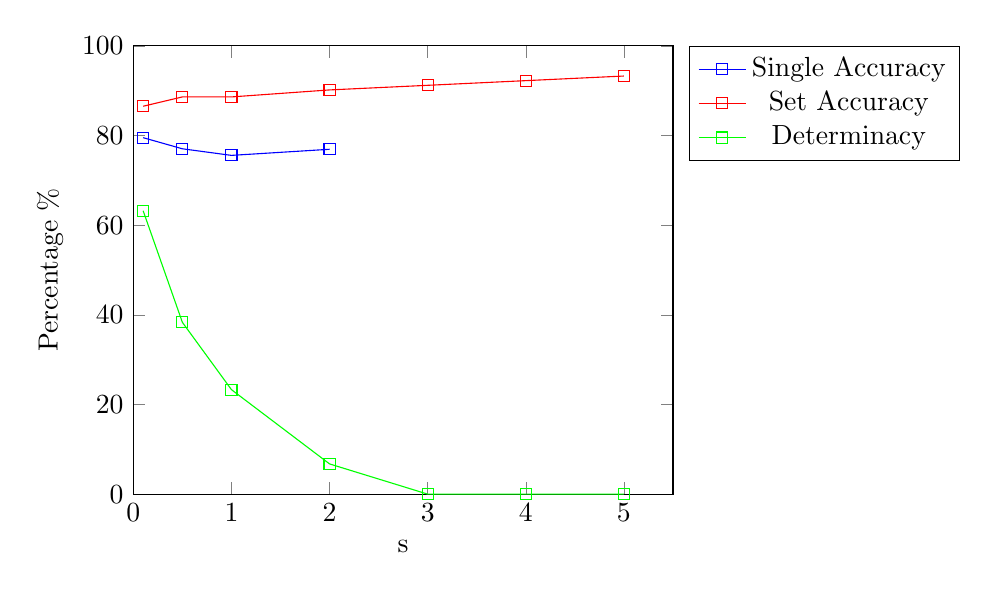
\begin{tikzpicture}
\begin{axis}[
    xlabel={s},
    ylabel={Percentage \%},
    xmin=0, xmax=5.5,
    ymin=0, ymax=100,
	legend pos=outer north east
]

\addplot[
    color=blue,
    mark=square,
    ]
    coordinates {
    (0.1,79.51)(0.5,77.03)(1,75.56)(2,76.92)
    };
    \label{sng_acc}

\addplot[
    color=red,
    mark=square,
    ]
    coordinates {
    (0.1,86.52)(0.5,88.60)(1,88.60)(2,90.16)(3, 91.19)(4, 92.23)(5,93.26)
    };
    \label{set_acc}
 
\addplot[
    color=green,
    mark=square,
    ]
    coordinates {
    (0.1,63.21)(0.5,38.32)(1,23.31)(2,6.74)(3, 0)(4, 0)(5,0)
    };
    \label{det}

\addlegendimage{/pgfplots/refstyle=sng_acc}\addlegendentry{Single Accuracy}
\addlegendimage{/pgfplots/refstyle=set_acc}\addlegendentry{Set Accuracy}
\addlegendimage{/pgfplots/refstyle=det}\addlegendentry{Determinacy}
\end{axis}

\end{tikzpicture}

Additionally we have the following measurements for indeterminate output size:
\begin{center}
\begin{tabular}{c|c c c c}
s & 0.5 & 1 & 2 & 5 \\
\hline
Indeterminate Output Size & 3.65 & 3.66 & 3.74 & 4.25
\end{tabular}
\end{center}

First we note the increase in indeterminate output size and decrease in determinacy.
These are due to the domination criteria becoming harder to satisfy for larger $s$ values.
This leads to less classes being credally dominated and larger output size.

This can also explain the slight trends in single and set accuracy.
Set accuracy increases because the indeterminate output size is always increasing so for each increase in $s$ value we are more likely to see the true class added to the oupur set if it was not already there.
On the other hand the single accuracy does not change much.
As we increase the $s$ value we decrease the number of single outputs and it would appear the outputs that become indeterminate are equally likely to be correct classifications as incorrect classifications.

We can also directly compare the classifications of the naive Credal classifier to those of our interval based classifier. For $s=1$ we have:
\begin{center}
\begin{tabular}{l|c c c c}
         & A\%     & B\%     & C    & D\%     \\
\hline
Interval & 75.61\% & 89.12\% & 3.71 & 21.32\% \\
NCC      & 75.56\% & 88.60\% & 3.66 & 23.31\% \\
\end{tabular}
\end{center}
Here we see similar set and single accuracies.
However we see that the naive Credal classifier is more determinate than the interval based classifier and, when indeterminate, has a smaller average output size.

Our data set only contains observations of three vehicles with risk rating -2.
This means that our credal classifiers struggle to eliminate this classification as an option.
When we consider situations where the NCC is indeterminate and returns two possible classes -2 is always one of these classes.
Additionally the other class is the correct classification 88.60\%.
This is a good example of a situation where the NCC reserves judgement due to lack of observations.

\bibliography{refs}{}
\bibliographystyle{plain}

\end{document}